% Options for packages loaded elsewhere
\PassOptionsToPackage{unicode}{hyperref}
\PassOptionsToPackage{hyphens}{url}
%
\documentclass[
]{article}
\usepackage{amsmath,amssymb}
\usepackage{iftex}
\ifPDFTeX
  \usepackage[T1]{fontenc}
  \usepackage[utf8]{inputenc}
  \usepackage{textcomp} % provide euro and other symbols
\else % if luatex or xetex
  \usepackage{unicode-math} % this also loads fontspec
  \defaultfontfeatures{Scale=MatchLowercase}
  \defaultfontfeatures[\rmfamily]{Ligatures=TeX,Scale=1}
\fi
\usepackage{lmodern}
\ifPDFTeX\else
  % xetex/luatex font selection
\fi
% Use upquote if available, for straight quotes in verbatim environments
\IfFileExists{upquote.sty}{\usepackage{upquote}}{}
\IfFileExists{microtype.sty}{% use microtype if available
  \usepackage[]{microtype}
  \UseMicrotypeSet[protrusion]{basicmath} % disable protrusion for tt fonts
}{}
\makeatletter
\@ifundefined{KOMAClassName}{% if non-KOMA class
  \IfFileExists{parskip.sty}{%
    \usepackage{parskip}
  }{% else
    \setlength{\parindent}{0pt}
    \setlength{\parskip}{6pt plus 2pt minus 1pt}}
}{% if KOMA class
  \KOMAoptions{parskip=half}}
\makeatother
\usepackage{xcolor}
\usepackage[margin=1in]{geometry}
\usepackage{color}
\usepackage{fancyvrb}
\newcommand{\VerbBar}{|}
\newcommand{\VERB}{\Verb[commandchars=\\\{\}]}
\DefineVerbatimEnvironment{Highlighting}{Verbatim}{commandchars=\\\{\}}
% Add ',fontsize=\small' for more characters per line
\usepackage{framed}
\definecolor{shadecolor}{RGB}{248,248,248}
\newenvironment{Shaded}{\begin{snugshade}}{\end{snugshade}}
\newcommand{\AlertTok}[1]{\textcolor[rgb]{0.94,0.16,0.16}{#1}}
\newcommand{\AnnotationTok}[1]{\textcolor[rgb]{0.56,0.35,0.01}{\textbf{\textit{#1}}}}
\newcommand{\AttributeTok}[1]{\textcolor[rgb]{0.13,0.29,0.53}{#1}}
\newcommand{\BaseNTok}[1]{\textcolor[rgb]{0.00,0.00,0.81}{#1}}
\newcommand{\BuiltInTok}[1]{#1}
\newcommand{\CharTok}[1]{\textcolor[rgb]{0.31,0.60,0.02}{#1}}
\newcommand{\CommentTok}[1]{\textcolor[rgb]{0.56,0.35,0.01}{\textit{#1}}}
\newcommand{\CommentVarTok}[1]{\textcolor[rgb]{0.56,0.35,0.01}{\textbf{\textit{#1}}}}
\newcommand{\ConstantTok}[1]{\textcolor[rgb]{0.56,0.35,0.01}{#1}}
\newcommand{\ControlFlowTok}[1]{\textcolor[rgb]{0.13,0.29,0.53}{\textbf{#1}}}
\newcommand{\DataTypeTok}[1]{\textcolor[rgb]{0.13,0.29,0.53}{#1}}
\newcommand{\DecValTok}[1]{\textcolor[rgb]{0.00,0.00,0.81}{#1}}
\newcommand{\DocumentationTok}[1]{\textcolor[rgb]{0.56,0.35,0.01}{\textbf{\textit{#1}}}}
\newcommand{\ErrorTok}[1]{\textcolor[rgb]{0.64,0.00,0.00}{\textbf{#1}}}
\newcommand{\ExtensionTok}[1]{#1}
\newcommand{\FloatTok}[1]{\textcolor[rgb]{0.00,0.00,0.81}{#1}}
\newcommand{\FunctionTok}[1]{\textcolor[rgb]{0.13,0.29,0.53}{\textbf{#1}}}
\newcommand{\ImportTok}[1]{#1}
\newcommand{\InformationTok}[1]{\textcolor[rgb]{0.56,0.35,0.01}{\textbf{\textit{#1}}}}
\newcommand{\KeywordTok}[1]{\textcolor[rgb]{0.13,0.29,0.53}{\textbf{#1}}}
\newcommand{\NormalTok}[1]{#1}
\newcommand{\OperatorTok}[1]{\textcolor[rgb]{0.81,0.36,0.00}{\textbf{#1}}}
\newcommand{\OtherTok}[1]{\textcolor[rgb]{0.56,0.35,0.01}{#1}}
\newcommand{\PreprocessorTok}[1]{\textcolor[rgb]{0.56,0.35,0.01}{\textit{#1}}}
\newcommand{\RegionMarkerTok}[1]{#1}
\newcommand{\SpecialCharTok}[1]{\textcolor[rgb]{0.81,0.36,0.00}{\textbf{#1}}}
\newcommand{\SpecialStringTok}[1]{\textcolor[rgb]{0.31,0.60,0.02}{#1}}
\newcommand{\StringTok}[1]{\textcolor[rgb]{0.31,0.60,0.02}{#1}}
\newcommand{\VariableTok}[1]{\textcolor[rgb]{0.00,0.00,0.00}{#1}}
\newcommand{\VerbatimStringTok}[1]{\textcolor[rgb]{0.31,0.60,0.02}{#1}}
\newcommand{\WarningTok}[1]{\textcolor[rgb]{0.56,0.35,0.01}{\textbf{\textit{#1}}}}
\usepackage{graphicx}
\makeatletter
\def\maxwidth{\ifdim\Gin@nat@width>\linewidth\linewidth\else\Gin@nat@width\fi}
\def\maxheight{\ifdim\Gin@nat@height>\textheight\textheight\else\Gin@nat@height\fi}
\makeatother
% Scale images if necessary, so that they will not overflow the page
% margins by default, and it is still possible to overwrite the defaults
% using explicit options in \includegraphics[width, height, ...]{}
\setkeys{Gin}{width=\maxwidth,height=\maxheight,keepaspectratio}
% Set default figure placement to htbp
\makeatletter
\def\fps@figure{htbp}
\makeatother
\setlength{\emergencystretch}{3em} % prevent overfull lines
\providecommand{\tightlist}{%
  \setlength{\itemsep}{0pt}\setlength{\parskip}{0pt}}
\setcounter{secnumdepth}{-\maxdimen} % remove section numbering
\ifLuaTeX
  \usepackage{selnolig}  % disable illegal ligatures
\fi
\IfFileExists{bookmark.sty}{\usepackage{bookmark}}{\usepackage{hyperref}}
\IfFileExists{xurl.sty}{\usepackage{xurl}}{} % add URL line breaks if available
\urlstyle{same}
\hypersetup{
  pdftitle={Lab\_06},
  pdfauthor={izd3},
  hidelinks,
  pdfcreator={LaTeX via pandoc}}

\title{Lab\_06}
\author{izd3}
\date{}

\begin{document}
\maketitle

Use only commands \& functions that are shown in the indicated chapter
or prior chapters.

\newpage

\hypertarget{problem-01---chapter-25-exercise-7}{%
\subsection{Problem \#01 - Chapter 25 Exercise
\#7}\label{problem-01---chapter-25-exercise-7}}

\begin{Shaded}
\begin{Highlighting}[]
\CommentTok{\# Show your work here}
\NormalTok{first\_10}\OtherTok{\textless{}{-}}\NormalTok{LETTERS[}\DecValTok{1}\SpecialCharTok{:}\DecValTok{10}\NormalTok{]}
\FunctionTok{sample}\NormalTok{(first\_10, }\DecValTok{3}\NormalTok{, }\AttributeTok{replace =} \ConstantTok{TRUE}\NormalTok{)}
\end{Highlighting}
\end{Shaded}

\begin{verbatim}
## [1] "E" "B" "J"
\end{verbatim}

\newpage

\hypertarget{problem-02---chapter-27-exercise-3}{%
\subsection{Problem \#02 - Chapter 27 Exercise
\#3}\label{problem-02---chapter-27-exercise-3}}

\begin{Shaded}
\begin{Highlighting}[]
\CommentTok{\# Show your work here}
\FunctionTok{library}\NormalTok{(}\StringTok{\textquotesingle{}patchwork\textquotesingle{}}\NormalTok{)}
\NormalTok{(patchwork01}\SpecialCharTok{|}\NormalTok{patchwork02)}\SpecialCharTok{/}\NormalTok{(patchwork01}\SpecialCharTok{|}\NormalTok{patchwork03}\SpecialCharTok{|}\NormalTok{patchwork04)}
\end{Highlighting}
\end{Shaded}

\includegraphics[height=300]{3040_Lab06_izd3_files/figure-latex/unnamed-chunk-2-1}

\newpage

\hypertarget{problem-03---chapter-28-exercise-2a}{%
\subsection{Problem \#03 - Chapter 28 Exercise
\#2A}\label{problem-03---chapter-28-exercise-2a}}

\begin{Shaded}
\begin{Highlighting}[]
\CommentTok{\# Show your work here}
\FunctionTok{library}\NormalTok{(}\StringTok{\textquotesingle{}ggplot2\textquotesingle{}}\NormalTok{)}
\end{Highlighting}
\end{Shaded}

\begin{verbatim}
## Warning: package 'ggplot2' was built under R version 4.2.3
\end{verbatim}

\begin{Shaded}
\begin{Highlighting}[]
\NormalTok{plot\_1}\OtherTok{\textless{}{-}}\FunctionTok{ggplot}\NormalTok{(}\AttributeTok{x=}\NormalTok{ggplot001.tib,}\AttributeTok{mapping =} \FunctionTok{aes}\NormalTok{(}\AttributeTok{x=}\NormalTok{ggplot001.tib}\SpecialCharTok{$}\NormalTok{var}\FloatTok{.1}\NormalTok{,}\AttributeTok{y=}\NormalTok{ggplot001.tib}\SpecialCharTok{$}\NormalTok{var}\FloatTok{.2}\NormalTok{,}\AttributeTok{color=}\NormalTok{ggplot001.tib}\SpecialCharTok{$}\NormalTok{group.var}\FloatTok{.1}\NormalTok{))}\SpecialCharTok{+}
  \FunctionTok{geom\_point}\NormalTok{(}\AttributeTok{size=}\DecValTok{4}\NormalTok{)}
\NormalTok{plot\_1}
\end{Highlighting}
\end{Shaded}

\includegraphics[height=300]{3040_Lab06_izd3_files/figure-latex/unnamed-chunk-3-1}

\newpage

\hypertarget{problem-0v4---chapter-28-exercise-4a-look-at-the-legends-to-help-determine-the-datasets-used.}{%
\subsection{Problem \#0v4 - Chapter 28 Exercise \#4A ( look at the
legends to help determine the datasets
used.)}\label{problem-0v4---chapter-28-exercise-4a-look-at-the-legends-to-help-determine-the-datasets-used.}}

\begin{Shaded}
\begin{Highlighting}[]
\CommentTok{\# Show your work here}
\NormalTok{plot\_1}\OtherTok{\textless{}{-}}\FunctionTok{ggplot}\NormalTok{(}\AttributeTok{x=}\NormalTok{ggplot001.tib,}\AttributeTok{mapping =} \FunctionTok{aes}\NormalTok{(}\AttributeTok{x=}\NormalTok{ggplot001.tib}\SpecialCharTok{$}\NormalTok{var}\FloatTok{.1}\NormalTok{,}\AttributeTok{y=}\NormalTok{ggplot001.tib}\SpecialCharTok{$}\NormalTok{var}\FloatTok{.2}\NormalTok{,}\AttributeTok{color=}\NormalTok{ggplot001.tib}\SpecialCharTok{$}\NormalTok{group.var}\FloatTok{.1}\NormalTok{))}\SpecialCharTok{+}
  \FunctionTok{geom\_point}\NormalTok{(}\AttributeTok{size=}\DecValTok{0}\NormalTok{)}

\NormalTok{plot\_1}\SpecialCharTok{+}\FunctionTok{geom\_point}\NormalTok{(}\AttributeTok{data =}\NormalTok{ ggplot001.tib,}\AttributeTok{size=}\DecValTok{4}\NormalTok{,}\AttributeTok{shape=}\DecValTok{6}\NormalTok{)}
\end{Highlighting}
\end{Shaded}

\begin{verbatim}
## Warning: Use of `ggplot001.tib$var.1` is discouraged.
## i Use `var.1` instead.
\end{verbatim}

\begin{verbatim}
## Warning: Use of `ggplot001.tib$var.2` is discouraged.
## i Use `var.2` instead.
\end{verbatim}

\begin{verbatim}
## Warning: Use of `ggplot001.tib$group.var.1` is discouraged.
## i Use `group.var.1` instead.
\end{verbatim}

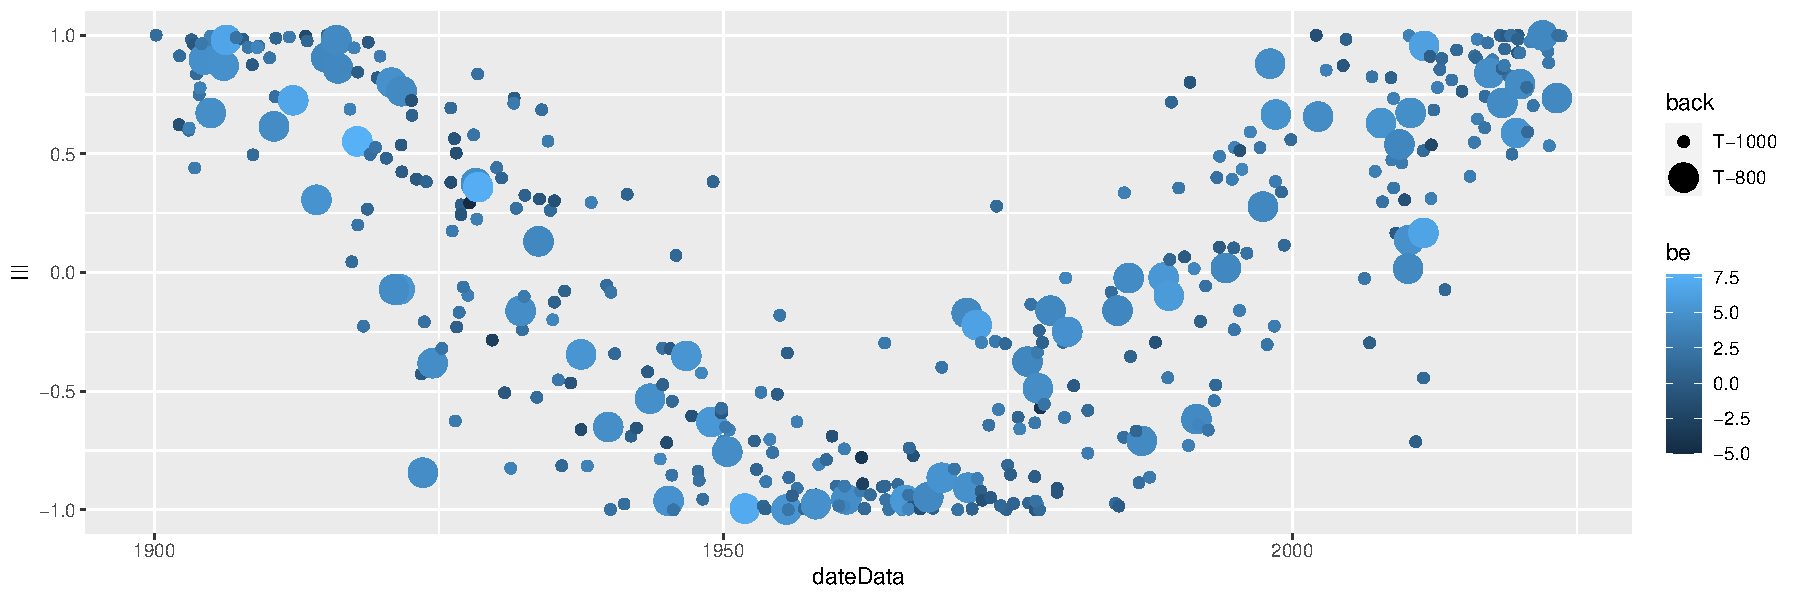
\includegraphics[height=300]{3040_Lab06_izd3_files/figure-latex/unnamed-chunk-4-1}

\end{document}
